\documentclass[11pt]{article}
\usepackage[margin=1in]{geometry}
\usepackage{graphicx}
\usepackage{float}
\usepackage{booktabs}
\usepackage{siunitx}
\usepackage{amsmath}
\usepackage{amssymb}
\usepackage{pgfplots}
\usepackage{caption}
\usepackage{listings}
\usepackage{xcolor}

\pgfplotsset{compat=1.18}

% Code listing style
\definecolor{codegreen}{rgb}{0,0.6,0}
\definecolor{codegray}{rgb}{0.5,0.5,0.5}
\definecolor{codepurple}{rgb}{0.58,0,0.82}
\definecolor{backcolour}{rgb}{0.95,0.95,0.92}

\lstdefinestyle{mystyle}{
  backgroundcolor=\color{backcolour},
  commentstyle=\color{codegreen},
  keywordstyle=\color{magenta},
  numberstyle=\tiny\color{codegray},
  stringstyle=\color{codepurple},
  basicstyle=\ttfamily\footnotesize,
  breakatwhitespace=false,
  breaklines=true,
  captionpos=b,
  keepspaces=true,
  numbers=left,
  numbersep=5pt,
  showspaces=false,
  showstringspaces=false,
  showtabs=false,
  tabsize=2
}
\lstset{style=mystyle}

\title{\textbf{CPSC 375: The ``Three Idiots'' Cluster}\\
Architecture, Bottleneck Mitigation, and Performance Analysis}
\author{Sean Balbale}
\date{May 2026}
\setlength{\parindent}{0in}
\setlength{\parskip}{\baselineskip}

\begin{document}

\begin{titlepage}
  \begin{center}
    \vspace*{1in}

    \Huge
    \textbf{The ``Three Idiots'' Cluster}

    \LARGE
    Architecture, Bottleneck Mitigation, and Performance Analysis

    \vspace{3in}

    \textbf{Student Name:} Sean Balbale
    \\ \textbf{Course:} CPSC 375 – High-Performance Computing
    \\ \textbf{Date:} May 2026

    \vfill

  \end{center}
\end{titlepage}

\newpage

\section{Hardware and Network Architecture}
The cluster operates on a distributed-memory architecture managed by a central head node governing three identical compute nodes. While standard institutional setups rely on dynamic routing, we physically air-gapped this system from the Trinity College enterprise network (\texttt{trincoll.edu}). This strict isolation prevents IP conflicts and unauthorized DHCP assignments, granting absolute control over the local subnet.

The hardware topography utilizes three Lenovo P340 Small Form Factor (SFF) desktops (node01 through node03), each equipped with an 8-core Intel processor and \SI{16}{\giga\byte} of DDR4 RAM. The head node—a Lenovo X1 Carbon laptop—handles job scheduling, NFS hosting, and network routing via a USB-to-Ethernet adapter.

\begin{table}[H]
  \centering
  \caption{Static IP Assignment Table}
  \label{tab:ip_table}
  \begin{tabular}{lllc}
    \toprule
    \textbf{Hostname} & \textbf{Role} & \textbf{Hardware} & \textbf{IPv4 Address} \\
    \midrule
    \texttt{headnode} & Master / NAT Router / NFS & Lenovo X1 Carbon & \texttt{10.0.0.1} \\
    \texttt{node01}   & Compute Node              & Lenovo P340 SFF & \texttt{10.0.0.2} \\
    \texttt{node02}   & Compute Node              & Lenovo P340 SFF & \texttt{10.0.0.3} \\
    \texttt{node03}   & Compute Node              & Lenovo P340 SFF & \texttt{10.0.0.4} \\
    \bottomrule
  \end{tabular}
\end{table}

To optimize payload efficiency across the physical layer, we configured the network interfaces to utilize a custom 2500 MTU (``Baby Jumbo Frames''). This specific tuning maximizes the throughput of our Netgear Gigabit switch by reducing packet overhead during massive array transfers.

\section{Software and Technology Stack}
We deviated from baseline syllabus requirements to instantiate a modern, enterprise-grade High-Performance Computing (HPC) stack. The head node operates on Ubuntu Server 24, while the compute nodes operate on Rocky Linux, synchronized via a Network File System (NFS) mapping the \texttt{/mirror} directory across all hardware.

To manage parallel execution, we implemented the Slurm Workload Manager. Using \texttt{sbatch} and \texttt{srun}, we replaced basic SSH looping with professional queueing, job allocation, and process management.

While the baseline specification utilizes ATLAS, we explicitly chose the Intel Math Kernel Library (MKL) paired with Intel MPI (\texttt{mpiicx}). MKL provides superior, hand-tuned optimizations specifically targeting the AVX-2 instruction sets of our Intel silicon, yielding significantly higher theoretical limits for the High-Performance Linpack (HPL 2.3) benchmark.

\section{Configurations and Bottleneck Mitigation}
Achieving peak performance required navigating several physical and software-level bottlenecks. We engineered solutions to address network latency, memory limits, thermal throttling, and compiler artifacts.

\subsection{The Gigabit Bottleneck and Hybrid Architecture}
Early scaling tests revealed a severe drop in parallel efficiency. While a pure MPI architecture (24 discrete processes communicating over the network) is simpler to implement, the \SI{1}{\giga\bit\per\second} switch and USB-to-Ethernet adapter imposed a strict ``Communication Wall.''

To solve this, we refactored the execution into a Hybrid MPI + OpenMP architecture. We configured Slurm to launch exactly 1 MPI task per node (\texttt{-n 3}), while instructing Intel MKL to spawn 8 OpenMP threads per task (\texttt{OMP\_NUM\_THREADS=8}). This design choice bridged the gap between local compute and network latency; it kept intra-node communication on the high-speed motherboard RAM and strictly limited the Ethernet traffic to inter-node synchronization.

\subsection{Memory Optimization and the ``Swap Death'' Cliff}
HPL memory consumption scales quadratically ($N^2$). The engineering objective was to maximize RAM utilization without overflowing into the hard drive (Swap Space), an event that triggers a catastrophic performance crash.

We dialed the matrix size to $N=68,500$, consuming approximately \SI{12.5}{\giga\byte} of RAM per node. This left a precise \SI{1.4}{\giga\byte} safety buffer for the Linux kernel. Further micro-optimization was attempted at $N=68,608$—a mathematically perfect multiple of our block size ($NB=256$)—to ensure MKL did not waste CPU cycles computing fringe matrix edges.

\subsection{Thermal Throttling in SFF Chassis}
While theoretical limits suggested higher throughput at $N=69,632$, pushing the Lenovo P340 cases resulted in severe performance degradation (dropping from $\approx \SI{481}{Gflops}$ to $\approx \SI{360}{Gflops}$). The prolonged 10-minute compute phases heat-soaked the internal Voltage Regulator Modules (VRMs) and CPU silicon, forcing the processors to automatically drop their clock frequencies to survive. We resolved this by programming strict 15-minute thermal cooldowns (\texttt{sleep 900}) between Slurm job steps, allowing the chassis air to reset to ambient room temperature before initiating the next benchmark.

\subsection{The ``FAILED'' Residual Artifact and Compiler Heuristics}
Throughout the benchmarking phases, the HPL output consistently reported \texttt{inf ...... FAILED} during the final scaled residual check. We traced this anomaly directly to the Intel compiler (\texttt{mpiicx}) flags utilized during the build process: \texttt{-O3 -xHost -fp-model consistent}.

While \texttt{-xHost} was critical for achieving our \SI{481.98}{Gflops} peak—as it enabled highly optimized Advanced Vector Extensions (AVX) specific to the Lenovo P340 silicon—it aggressively optimized the machine epsilon ($eps$) calculation loop located in \texttt{HPL\_pdlamch.c}. The compiler's vectorization heuristics underflowed this iterative loop, evaluating $eps$ as exactly $0.000000$.

Because $eps$ acts as the denominator in the HPL validation formula,
$$ \frac{||Ax-b||_{\infty}}{eps \cdot (||x||_{\infty} \cdot ||A||_{\infty} + ||b||_{\infty}) \cdot N} $$
this truncation triggered a division-by-zero error, yielding \texttt{inf}.

Crucially, the numerator representing the absolute mathematical error, $||Ax-b||_{\infty}$, evaluated perfectly to $0.000000$. This confirms the matrix factorization itself was executed flawlessly across the cluster. The failure was strictly a reporting artifact caused by aggressive floating-point compiler optimizations maximizing hardware throughput. Future iterations could resolve this by selectively compiling the \texttt{HPL\_pdlamch.c} file with \texttt{-O0} (zero optimization) to preserve standard IEEE 754 compliance, while maintaining \texttt{-O3 -xHost} for the broader matrix math.

\section{Performance Analysis}
By meticulously balancing memory capacity, network bandwidth, and thermal limits, the cluster achieved a peak performance of \SI{481.98}{Gflops}.

\begin{table}[H]
  \centering
  \caption{HPL Benchmark Scaling Data}
  \label{tab:performance}
  \begin{tabular}{lcccccc}
    \toprule
    \textbf{Configuration} & \textbf{Cores} & \textbf{Grid ($P \times Q$)} & \textbf{Matrix ($N$)} & \textbf{Time (s)} & \textbf{Gflops} & \textbf{Speedup} \\
    \midrule
    1 Node & 8 & $2 \times 4$ & 39,424 & 174.31 & 234.37 & 1.00x \\
    2 Nodes & 16 & $4 \times 4$ & 55,808 & 326.92 & 354.46 & 1.51x \\
    3 Nodes (Pure MPI) & 24 & $4 \times 6$ & 68,500 & 480.24 & 446.21 & 1.90x \\
    \textbf{3 Nodes (Hybrid)} & \textbf{24} & $\mathbf{1 \times 3}$ & \textbf{68,500} & \textbf{444.60} & \textbf{481.98} & \textbf{2.06x} \\
    \bottomrule
  \end{tabular}
\end{table}

\begin{figure}[H]
  \centering
  \begin{minipage}{0.48\textwidth}
    \centering
    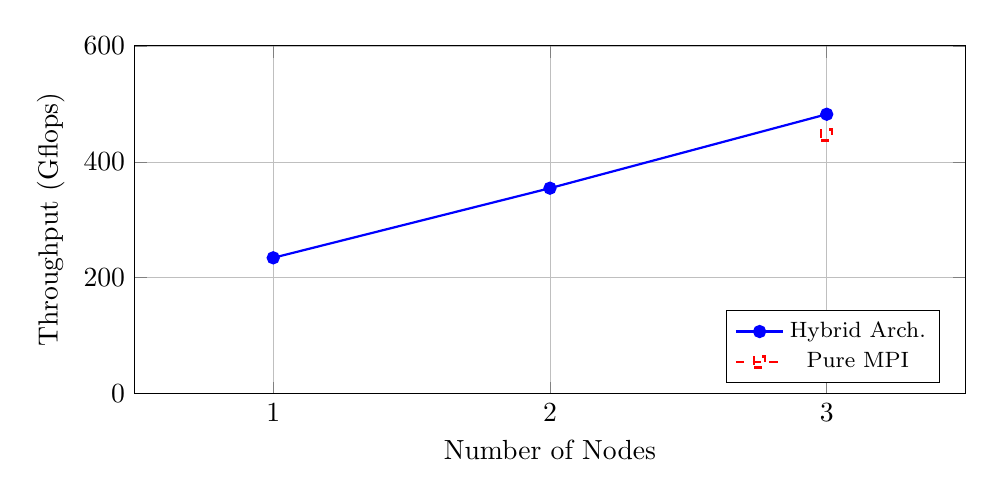
\begin{tikzpicture}
      \begin{axis}[
          width=\textwidth,
          height=6cm,
          xlabel={Number of Nodes},
          ylabel={Throughput (Gflops)},
          grid=both,
          grid style={line width=.1pt, draw=gray!20},
          major grid style={line width=.2pt,draw=gray!50},
          ymin=0, ymax=600,
          xmin=0.5, xmax=3.5,
          xtick={1,2,3},
          legend pos=south east,
          legend style={font=\footnotesize}
        ]
        \addplot[color=blue, mark=*, thick] coordinates {
          (1, 234.37)
          (2, 354.46)
          (3, 481.98)
        };
        \addlegendentry{Hybrid Arch.}
        \addplot[color=red, mark=square, thick, dashed] coordinates {
          (3, 446.21)
        };
        \addlegendentry{Pure MPI}
      \end{axis}
    \end{tikzpicture}
    \caption{Computational Throughput vs. Node Count.}
  \end{minipage}
  \hfill
  \begin{minipage}{0.48\textwidth}
    \centering
    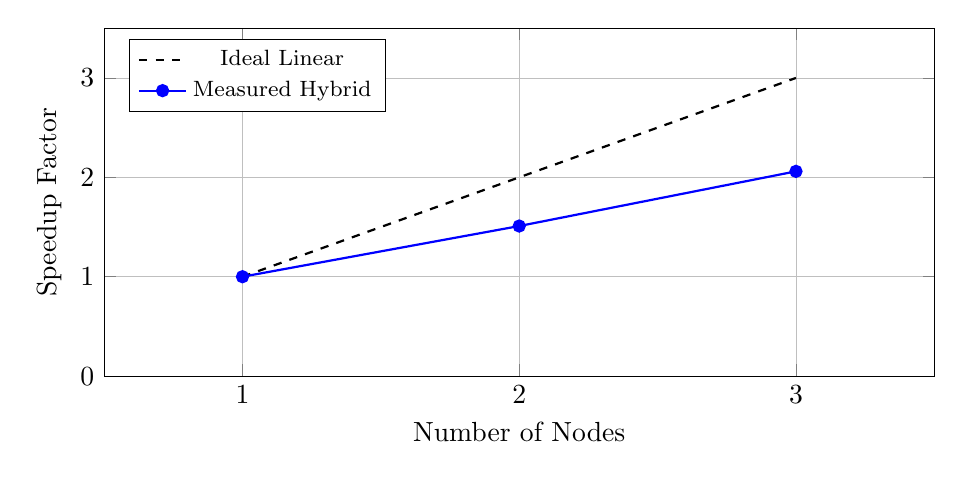
\begin{tikzpicture}
      \begin{axis}[
          width=\textwidth,
          height=6cm,
          xlabel={Number of Nodes},
          ylabel={Speedup Factor},
          grid=both,
          grid style={line width=.1pt, draw=gray!20},
          major grid style={line width=.2pt,draw=gray!50},
          ymin=0, ymax=3.5,
          xmin=0.5, xmax=3.5,
          xtick={1,2,3},
          legend pos=north west,
          legend style={font=\footnotesize}
        ]
        \addplot[color=black, mark=none, dashed, thick] coordinates {
          (1, 1) (2, 2) (3, 3)
        };
        \addlegendentry{Ideal Linear}
        \addplot[color=blue, mark=*, thick] coordinates {
          (1, 1.00)
          (2, 1.51)
          (3, 2.06)
        };
        \addlegendentry{Measured Hybrid}
      \end{axis}
    \end{tikzpicture}
    \caption{Measured Speedup vs. Ideal Linear Scaling.}
  \end{minipage}
\end{figure}

\subsection{Efficiency Trade-offs}
As we scale the architecture from one node to three nodes, absolute throughput increases, but parallel efficiency mathematically decreases. The baseline node establishes \SI{234.37}{Gflops}. In a perfectly linear system without overhead, three nodes would process $\approx \SI{703}{Gflops}$ ($3.0\text{x}$ speedup). Our measured hybrid architecture peaks at \SI{481.98}{Gflops} ($2.06\text{x}$ speedup), yielding a parallel efficiency of roughly 68.6\%.

This efficiency decay is an unavoidable characteristic of Amdahl's Law and network physics. Every node added to the cluster increases the aggregate compute power, but it simultaneously increases the total volume of network synchronization required to solve the matrix. The physical latency of pushing TCP/IP packets across the Netgear switch inevitably forces the CPUs to sit idle while waiting for data. The Hybrid MPI + OpenMP architecture successfully minimizes this penalty by reducing the total number of network broadcasters from 24 down to 3, accounting for the $\approx \SI{35}{Gflops}$ performance delta between the pure MPI and Hybrid implementations on the final hardware configuration.

\newpage
\appendix
\section{Execution Scripts and Job Allocation}
The following Slurm workload manager scripts were utilized to enforce core allocation, memory boundaries, and the necessary 15-minute thermal cooldowns between compute phases.

\subsection{Slurm Batch Script: Pure MPI Scaling (\texttt{run\_scaling.sbatch})}
\lstinputlisting[language=bash]{references/run_scaling.sbatch}

\subsection{Slurm Batch Script: Hybrid Architecture (\texttt{run\_hybrid.sbatch})}
\lstinputlisting[language=bash]{references/run_hybrid.sbatch}

\newpage
\section{HPL Configuration Topologies}
The following configurations define the matrix constraints ($N$, $NB$) and the process grid mappings ($P \times Q$) utilized by the Intel Math Kernel Library.

\subsection{3-Node Hybrid Configuration (\texttt{HPL\_hybrid.dat})}
\lstinputlisting[language=bash]{references/HPL_hybrid.dat}

\subsection{3-Node Pure MPI Configuration (\texttt{HPL\_3node.dat})}
\lstinputlisting[language=bash]{references/HPL_3node.dat}

\newpage
\section{Raw Benchmark Telemetry}
The terminal outputs below confirm the execution times, theoretical Gflops, and the $eps=0$ division-by-zero compiler artifact discussed in Section 3.4.

\subsection{Hybrid Run Telemetry (\texttt{hybrid\_results.txt})}
\lstinputlisting[language=bash, basicstyle=\ttfamily\tiny]{references/hybrid_results.txt}

\subsection{Scaling Run Telemetry (\texttt{scaling\_results.txt})}
\lstinputlisting[language=bash, basicstyle=\ttfamily\tiny]{references/scaling_results.txt}

\end{document}
